\documentclass[10pt,letterpaper]{article}
\usepackage[T1]{fontenc}
\usepackage{newtxtext}
\renewcommand{\ttdefault}{lmtt}
\usepackage[left=0.62in,right=0.62in,top=0.55in,bottom=0.58in]{geometry}
\usepackage[hyphens]{url}
\usepackage{graphicx}
\graphicspath{{./}{../}}
\urlstyle{rm}
\def\UrlFont{\rm}
\usepackage[font=small,labelfont=bf,skip=4pt]{caption}
\frenchspacing

\usepackage{amsmath}
\usepackage{amssymb}
\usepackage{booktabs}
\usepackage{array}
\usepackage{placeins}

\setlength{\parindent}{1em}
\setlength{\parskip}{0pt}
\setlength{\textfloatsep}{8pt plus 2pt minus 2pt}
\setlength{\floatsep}{7pt plus 2pt minus 2pt}
\setlength{\intextsep}{7pt plus 2pt minus 2pt}
\setlength{\abovedisplayskip}{6pt plus 2pt minus 2pt}
\setlength{\belowdisplayskip}{6pt plus 2pt minus 2pt}
\setcounter{topnumber}{6}
\setcounter{bottomnumber}{4}
\setcounter{totalnumber}{8}
\renewcommand{\topfraction}{0.95}
\renewcommand{\bottomfraction}{0.90}
\renewcommand{\textfraction}{0.05}
\renewcommand{\floatpagefraction}{0.82}

\makeatletter
\renewcommand\section{\@startsection{section}{1}{0pt}%
  {1.5ex plus 0.5ex minus 0.2ex}{0.6ex}%
  {\normalfont\large\bfseries}}
\renewcommand\subsection{\@startsection{subsection}{2}{0pt}%
  {1.2ex plus 0.4ex minus 0.2ex}{0.4ex}%
  {\normalfont\normalsize\bfseries}}
\renewcommand\paragraph{\@startsection{paragraph}{4}{0pt}%
  {0.9ex plus 0.3ex minus 0.2ex}{-0.6em}%
  {\normalfont\normalsize\bfseries}}
% Legacy full-width tables become ordinary flexible floats in one-column mode.
\renewenvironment{table*}[1][tbp]
  {\begin{table}[!htbp]}
  {\end{table}}
\makeatother

\setcounter{secnumdepth}{2}

\begin{document}
\suppressfloats[t]
\begin{center}
{\LARGE\bfseries Technical Supplement}\\[2pt]
{\large\bfseries SABER: Support-Conditioned Bellman Error Reweighting\\
for Sparse-Reward Hindsight Experience Replay}\\[3pt]
{\normalsize Anonymous Submission}
\end{center}
\vspace{2pt}

\noindent\textbf{Overview.}
This supplement provides complete experimental settings, seed-level primary
results, sensitivity and scope controls, support-signal diagnostic details,
runtime measurements, and an index of the anonymous code-and-data artifacts.
It uses the terminology and method definitions of the main paper.

\noindent\textbf{Working-draft completion status.}
Two result slots are intentionally marked \emph{pending}: FPP DDPG
Actor+Critic and DrawerOpen DDPG fixed-target diagnostics. No value is
inferred from an incomplete run or from the earlier live-target diagnostic.
These markers and this paragraph must be removed only after complete,
validated artifacts have replaced both slots.

\section{Experimental and Reproducibility Details}

\subsection{Tasks, Cohorts, and Shared Training Settings}

Tables~\ref{tab:supp-task-cohorts}--\ref{tab:supp-backbone-settings} give the
settings shared within each matched cohort. The primary comparison contains
seven task--backbone cohorts and uses paired seeds 1--5. Drawer SAC is not a
primary cohort because a complete matched HER--SABER pair was not collected.

\begin{table*}[t]
\centering
\small
\setlength{\tabcolsep}{6pt}
\begin{tabular}{lllll}
\toprule
Task & Horizon & Budget & Backbones & Exact primary grid \\
\midrule
FetchPickAndPlace-v4 & 50 & 1M & DDPG, TD3, SAC & 10k (DDPG/TD3), 50k (SAC) \\
DrawerOpen & 200 & 2M & DDPG, TD3 & 10k \\
DrawerClose & 200 & 2M & DDPG, TD3 & 10k \\
\bottomrule
\end{tabular}
\caption{Primary task and cohort definitions. Every method within a
task--backbone cohort uses the same environment-step budget and exact
evaluation grid. Primary comparisons use paired seeds 1--5.}
\label{tab:supp-task-cohorts}
\end{table*}

\begin{table*}[t]
\centering
\small
\setlength{\tabcolsep}{5pt}
\begin{tabular}{ll}
\toprule
Setting & Value or convention \\
\midrule
HER & Future-goal convention in the main paper; nominal \(p_{\mathrm{HER}}=0.8\) \\
Replay & Uniform for HER and SABER; capacity 300k; minibatch size 256 \\
Networks & Actor and critic MLPs with two hidden layers of 256 units \\
Optimization & Adam, actor and critic learning rates \(3\times10^{-4}\) \\
Discount and targets & \(\gamma=0.98\), Polyak coefficient \(\tau=0.005\) \\
Update schedule & UTD 1; learning begins after 5k steps; random actions for first 10k steps \\
Termination & Successful relabeled transitions are nonterminal; time limits bootstrap \\
Evaluation & Deterministic policy, 20 episodes per checkpoint \\
Statistics & Seed mean and sample SD; paired percentile-bootstrap CI, 10,000 resamples, RNG seed 2027 \\
Curve processing & Exact common checkpoints only; no smoothing, interpolation, extrapolation, or filling \\
\bottomrule
\end{tabular}
\caption{Shared training, evaluation, and statistical settings. Matched
HER--SABER runs use identical replay and relabeling code.}
\label{tab:supp-shared-settings}
\end{table*}

\begin{table*}[t]
\centering
\small
\setlength{\tabcolsep}{6pt}
\begin{tabular}{llll}
\toprule
Backbone & Critic & Exploration or entropy & Backbone-specific settings \\
\midrule
DDPG & One critic & Gaussian action noise, SD \(0.2\) & Deterministic actor \\
TD3 & Twin critics & Gaussian action noise, SD \(0.2\) & Target noise \(0.2\), clip \(0.5\), policy delay 2 \\
SAC & Twin critics & Automatic entropy tuning & Initial \(\alpha=0.2\), \(\alpha\) LR \(3\times10^{-4}\), target entropy \(-4\) \\
\bottomrule
\end{tabular}
\caption{Backbone-specific settings. SABER preserves each backbone's target
construction and actor-update rule.}
\label{tab:supp-backbone-settings}
\end{table*}


\paragraph{HER convention.}
For an episode with transitions indexed by \(t=0,\ldots,T-1\), a transition
selected for relabeling samples
\[
u\sim\operatorname{Unif}\{t+1,\ldots,T-1\},\qquad
\widetilde g=m(s_{u+1}).
\]
The original desired goal is retained when the eligible set is empty or when
relabeling is not selected. Reward is recomputed using \(\widetilde g\).
Consequently, the nominal relabeling probability is \(0.8\), while the
realized fraction may be slightly lower near an episode boundary. Matched
HER--SABER cohorts execute the same replay and relabeling code.

\paragraph{Terminal convention.}
A successfully relabeled transition is treated as nonterminal for bootstrap
purposes. Time-limit transitions also bootstrap. This convention is identical
across methods within each cohort.

\paragraph{Development scope and seed mapping.}
We did not conduct an exhaustive joint hyperparameter search. The Main SABER
settings were fixed for the matched comparisons, and no control received
variant-specific tuning. The \(K\in\{3,7\}\) runs are reported as sensitivity
checks around Main \(K=5\), not as a per-task model-selection sweep. For paired
seed \(s\), the environment, PyTorch, NumPy, and action-noise streams use \(s\);
the support-weight stream uses \(20000+s\), and evaluation uses base seed
\(10000+s\). Training resets advance deterministically with the episode index,
and evaluation resets use a deterministic checkpoint- and episode-indexed
offset. All methods in a paired cohort use the same seed mapping.

\subsection{Support Context and Retrieval}

\begin{table*}[t]
\centering
\small
\setlength{\tabcolsep}{5pt}
\begin{tabular}{>{\raggedright\arraybackslash}p{0.16\textwidth}
                >{\raggedright\arraybackslash}p{0.43\textwidth}
                >{\raggedright\arraybackslash}p{0.32\textwidth}}
\toprule
Task family & Full context components & Coarse retrieval key \\
\midrule
FetchPickAndPlace & Phase, hand--object distance, object--goal distance,
object height, gripper gap, horizon & Hand--object distance, object height,
gripper gap, horizon \\
DrawerOpen/Close & Phase, hand--handle distance, handle--goal distance,
handle \(y\), gripper state, horizon & Hand--handle distance, handle \(y\),
gripper state, horizon \\
\bottomrule
\end{tabular}
\caption{Task-specific support contexts. Candidate retrieval uses the coarse
key, after which exact component-wise equality on the full discretized context
defines the local replay set.}
\label{tab:supp-context-components}
\end{table*}

\begin{table*}[t]
\centering
\small
\setlength{\tabcolsep}{4pt}
\begin{tabular}{>{\raggedright\arraybackslash}p{0.16\textwidth}
                >{\raggedright\arraybackslash}p{0.37\textwidth}
                >{\raggedright\arraybackslash}p{0.37\textwidth}}
\toprule
Component & FetchPickAndPlace thresholds & Drawer thresholds \\
\midrule
Phase & approach, grasp, lift, place & approach, contact, opening/closing, open/closed \\
Hand distance & \(.03,.05,.08,.12,.20,.40\) & \(.03,.05,.08,.12,.20,.40\) \\
Goal distance & \(.05,.10,.20,.40,.70\) & \(.03,.05,.08,.12,.20,.40,.70\) \\
Task coordinate & object \(z\): \(.43,.48,.55,.65,.75\) & handle \(y\): \(-.05,0,.05,.10,.15,.25\) \\
Gripper & gap: \(.02,.05,.08\) & state: \(-.50,0,.50\) \\
Remaining horizon & \(10,25,50,100\) & \(10,25,50,100,200,500\) \\
\bottomrule
\end{tabular}
\caption{Discretization boundaries used to construct support contexts. Values
are applied component-wise in environment units. The main method normalizes
each action dimension to its action bounds and uses \(K=5\) bins per
dimension, \(N_{\mathrm{scan}}=512\), \(N_{\mathrm{local}}=4\), and
\(\lambda_S=1\).}
\label{tab:supp-context-thresholds}
\end{table*}


The replay index returns at most \(N_{\mathrm{scan}}\) slots associated with a
coarse retrieval key in implementation-defined index order. Those candidates
are filtered by exact component-wise equality of the full context. The current
implementation does not guarantee temporal recency after circular-buffer
wraparound; no claim relies on candidates being the most recent transitions.
The sampled transition remains eligible to appear in its own local replay
set.

For the Drawer phase definitions, let \(d_h\) be hand--handle distance and
\(d_g\) be handle--goal distance. The terminal phase is open or closed when
\(d_g\leq0.05\); the opening or closing phase requires \(d_h\leq0.08\) and
\(0.05<d_g\leq0.12\); contact requires \(d_h\leq0.08\) and \(d_g>0.12\);
remaining samples are approach. Phases use the relabeled training goal.

\subsection{Comparison Methods}

\begin{table*}[t]
\centering
\small
\setlength{\tabcolsep}{5pt}
\begin{tabular}{llll}
\toprule
Method & Selection changed & Loss coefficient & Correction \\
\midrule
HER & None beyond uniform replay and HER relabeling & Uniform & None \\
SABER & None & Current-policy local-support weight & Unit minibatch mean \\
HGR & Episode and transition--future-goal pair & HGR importance weight & Two-stage IS \\
PER & Replay transition & PER importance weight & Annealed IS \\
TD-error weighting & None & TD-error-derived weight & Unit minibatch mean \\
\bottomrule
\end{tabular}
\caption{Operational intervention points. HGR uses priority exponents
\(\alpha_{\mathrm{episode}}=\alpha_{\mathrm{pair}}=0.6\), while PER uses
\(\alpha=0.6\). Both anneal \(\beta\) linearly from \(0.4\) to \(1.0\) over
critic-update progress and use priority offset \(10^{-6}\). TD-error weighting
retains uniform replay and is therefore the closest allocation-stage control.}
\label{tab:supp-comparison-settings}
\end{table*}


\paragraph{HGR.}
The implementation prioritizes an episode and then a transition--future-goal
pair. The two importance factors are multiplied and normalized on relabeled
samples; the original-goal branch retains coefficient one. The episode and
pair priority exponents are both \(0.6\).

\paragraph{PER.}
Replay transitions are sampled by TD-error priority with exponent \(0.6\).
The importance exponent increases linearly from \(0.4\) to \(1.0\) over the
training budget. PER changes realized minibatch membership, unlike SABER and
the TD-error critic-loss weighting control.

\paragraph{TD-error critic-loss weighting.}
This control preserves uniform replay and changes only normalized per-sample
critic coefficients. DDPG uses its single absolute TD error. SAC uses
\(\min(|\delta_{i1}|,|\delta_{i2}|)\) as the signal and applies the resulting
coefficient to both critic losses. TD3 results are not reported because the
stored control used independent target-policy smoothing noise for weight
construction and optimized residuals, preventing the intended matched-signal
interpretation.

\subsection{Metrics and Statistical Analysis}

Let \(q_j\in[0,1]\) be deterministic evaluation success at exact shared
checkpoint \(t_j\). Normalized success AUC is
\[
\operatorname{AUC}
=\frac{1}{t_m-t_1}
\sum_{j=1}^{m-1}
\frac{q_j+q_{j+1}}{2}(t_{j+1}-t_j).
\]
Final-quarter AUC applies the same calculation to 750k--1M for FPP and
1.5M--2M for Drawer tasks. Final success is the value at the final checkpoint.
Hit90 is the first exact checkpoint with \(q_j\geq0.9\); its median is
computed only over seeds that reach the threshold, so reached-seed coverage
is always reported.

For paired comparisons, each seed contributes one method difference. The
reported 95\% intervals are percentile intervals from 10,000 paired bootstrap
resamples with pseudorandom seed 2027. Sample standard deviations use
\(n-1\) in the denominator. No curve is smoothed, interpolated,
extrapolated, or forward-filled.

\FloatBarrier
\section{Primary Comparison Details}

\subsection{Drawer Learning Curves}

\begin{figure}[!tbp]
\centering
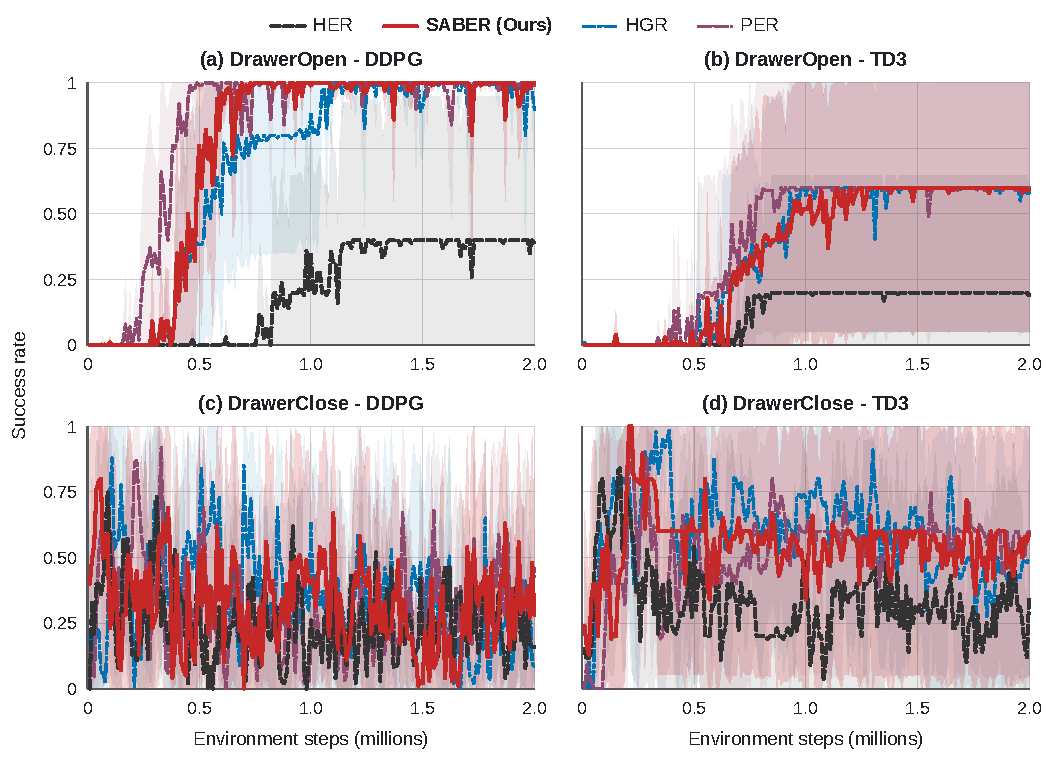
\includegraphics[width=\textwidth]{figures/supplementary_drawer_primary_learning_curves.pdf}
\caption{DrawerOpen and DrawerClose learning curves for DDPG and TD3.
Lines are seed means and bands are sample standard deviations over paired
seeds 1--5 on the exact 10k grid. No smoothing or interpolation is applied.}
\label{fig:supp-drawer-primary-curves}
\end{figure}

\FloatBarrier
\subsection{Time to Threshold}

% Supplementary time-to-threshold results for the primary comparisons.
\begin{table*}[t]
\centering
\small
\begin{tabular*}{\textwidth}{@{\extracolsep{\fill}}lllcc@{}}
\toprule
Task & Backbone & Method & Median Hit90 & Reached seeds \\
\midrule
FetchPickAndPlace & DDPG & SABER & 540k & 5/5 \\
 & & HER & 600k & 5/5 \\
 & & HGR & 930k & 2/5 \\
 & & PER & 640k & 4/5 \\
\addlinespace
FetchPickAndPlace & TD3 & SABER & 840k & 5/5 \\
 & & HER & 980k & 3/5 \\
 & & HGR & 630k & 1/5 \\
 & & PER & 1.00M & 1/5 \\
\addlinespace
FetchPickAndPlace & SAC & SABER & 750k & 5/5 \\
 & & HER & 800k & 3/5 \\
 & & HGR & 800k & 2/5 \\
 & & PER & 550k & 5/5 \\
\addlinespace
DrawerOpen & DDPG & SABER & 500k & 5/5 \\
 & & HER & 960k & 2/5 \\
 & & HGR & 530k & 5/5 \\
 & & PER & 330k & 5/5 \\
\addlinespace
DrawerOpen & TD3 & SABER & 780k & 3/5 \\
 & & HER & 740k & 1/5 \\
 & & HGR & 760k & 3/5 \\
 & & PER & 720k & 3/5 \\
\addlinespace
DrawerClose & DDPG & SABER & 20k & 5/5 \\
 & & HER & 70k & 5/5 \\
 & & HGR & 100k & 5/5 \\
 & & PER & 60k & 5/5 \\
\addlinespace
DrawerClose & TD3 & SABER & 80k & 5/5 \\
 & & HER & 70k & 5/5 \\
 & & HGR & 80k & 5/5 \\
 & & PER & 120k & 5/5 \\
\bottomrule
\end{tabular*}
\caption{Hit90 for the primary comparisons. Hit90 is the first exact-grid
checkpoint at which deterministic evaluation success reaches at least 0.9.
Medians use only reached seeds, so reached-seed coverage is reported
separately.}
\label{tab:supp-primary-hit90}
\end{table*}


Hit90 is a threshold-crossing summary rather than a stability measure.
Coverage is especially important when only a subset of seeds reaches 0.9.

\FloatBarrier
\subsection{FPP TD3 Confirmatory and HER-Indexing Sensitivity Results}

% Frozen FPP TD3 confirmatory extension. Values are generated from
% experiment_FPP/paper_artifacts/fpp_td3_her_vs_saber_n10_1m.
\begin{table}[t]
\centering
\small
\setlength{\tabcolsep}{5pt}
\begin{tabular}{@{}lccc@{}}
\toprule
Seed & HER AUC & SABER AUC & Difference \\
\midrule
1  & 0.3465 & 0.4301 & $+0.0836$ \\
2  & 0.3727 & 0.4568 & $+0.0841$ \\
3  & 0.3942 & 0.4960 & $+0.1018$ \\
4  & 0.4109 & 0.4066 & $-0.0043$ \\
5  & 0.3338 & 0.4225 & $+0.0886$ \\
6  & 0.4301 & 0.5207 & $+0.0907$ \\
7  & 0.3995 & 0.4614 & $+0.0619$ \\
8  & 0.3068 & 0.3543 & $+0.0475$ \\
9  & 0.4106 & 0.4114 & $+0.0008$ \\
10 & 0.4210 & 0.3331 & $-0.0879$ \\
\midrule
Mean & 0.3826 & 0.4293 & $+0.0467$ \\
\bottomrule
\end{tabular}
\caption{Frozen FPP TD3 confirmatory extension over ten paired seeds. AUC is
computed on the exact 10k--1M evaluation grid without smoothing,
interpolation, or filling. The paired mean difference is $+0.0467$
(10,000-resample paired-bootstrap 95\% CI $[0.0085,0.0783]$); 8/10 paired
differences are positive. The exact two-sided sign-flip test over all 1,024
assignments gives $p=0.0527$.}
\label{tab:supp-fpp-td3-n10}
\end{table}

% FPP TD3 inclusive-future sensitivity. This fragment is placed in the right
% minipage of the paired extension/sensitivity float.
\centering
\small
\setlength{\tabcolsep}{2.5pt}
\begin{tabular}{@{}rccc@{}}
\toprule
Seed & HER AUC & SABER (Ours) AUC & Difference \\
\midrule
1 & 0.3005 & 0.4576 & $+0.1571$ \\
2 & 0.2674 & 0.2669 & $-0.0005$ \\
3 & 0.3467 & 0.5179 & $+0.1712$ \\
4 & 0.3487 & 0.4003 & $+0.0515$ \\
5 & 0.3669 & 0.3247 & $-0.0422$ \\
6 & 0.3664 & 0.3404 & $-0.0260$ \\
7 & 0.4285 & 0.3449 & $-0.0836$ \\
8 & 0.3235 & 0.3076 & $-0.0159$ \\
9 & 0.1846 & 0.3535 & $+0.1689$ \\
10 & 0.3341 & 0.3475 & $+0.0134$ \\
\midrule
Mean & 0.3267 & 0.3661 & $+0.0394$ \\
\bottomrule
\end{tabular}
\captionof{table}{FPP TD3 inclusive-future sensitivity, also admitting
$m(s_{t+1})$, over ten paired seeds. Seeds 6--10 extend the original cohort;
the pooled AUC is descriptive and uses the exact 10k--1M grid.}
\label{tab:supp-fpp-td3-inclusive-future}


The ten-seed cohort extends the frozen primary FPP TD3 comparison. The
inclusive-future sensitivity also admits \(m(s_{t+1})\), while leaving the
matched HER--SABER difference otherwise unchanged. Its positive observed mean
direction does not constitute an equivalence test between HER indexing
conventions.

\FloatBarrier
\section{Additional Controls and Sensitivities}

\subsection{Allocation Signal}

% Supplementary allocation-signal control. TD3 cohorts are intentionally
% excluded because their weights and optimized residuals used independent
% target-policy smoothing noise.
\begin{table*}[t]
\centering
\begin{tabular*}{\textwidth}{@{\extracolsep{\fill}}lllccc@{}}
\toprule
Task & Backbone & Method & Final & AUC & Hit90 \\
\midrule
FetchPickAndPlace & DDPG & SABER & $0.960\pm0.042$ & $0.609\pm0.038$ & 540k (5/5) \\
FetchPickAndPlace & DDPG & TD-error & $0.930\pm0.104$ & $0.568\pm0.069$ & 630k (5/5) \\
\addlinespace
DrawerOpen & DDPG & SABER & $1.000\pm0.000$ & $0.754\pm0.044$ & 500k (5/5) \\
DrawerOpen & DDPG & TD-error & $0.800\pm0.447$ & $0.715\pm0.090$ & 610k (5/5) \\
\addlinespace
DrawerClose & DDPG & SABER & $0.280\pm0.251$ & $0.324\pm0.082$ & 20k (5/5) \\
DrawerClose & DDPG & TD-error & $0.400\pm0.166$ & $0.313\pm0.098$ & 130k (5/5) \\
\addlinespace
FetchPickAndPlace & SAC & SABER & $0.990\pm0.022$ & $0.583\pm0.030$ & 750k (5/5) \\
FetchPickAndPlace & SAC & TD-error & $0.990\pm0.022$ & $0.544\pm0.068$ & 800k (5/5) \\
\bottomrule
\end{tabular*}
\caption{Validated TD-error critic-loss weighting controls. Replay sampling
remains uniform, and only critic-loss coefficients are changed. Values are
mean $\pm$ sample standard deviation over paired seeds 1--5. SABER rows
reproduce the matched main-method values; TD-error rows use TD-error
critic-loss weighting.}
\label{tab:supp-td-error-weighting}
\end{table*}


Across the validated DDPG and SAC cohorts in
Table~\ref{tab:supp-td-error-weighting}, SABER has higher observed mean AUC
than TD-error critic-loss weighting. These controls isolate the weighting
signal more closely than PER because both retain uniform replay.

\FloatBarrier
\subsection{Action-Bin Resolution}

% Generated by paper/analysis/build_supplementary_results.py.
\begin{table*}[t]
\centering
\small
\setlength{\tabcolsep}{2pt}
\begin{tabular}{llccccccc}
\toprule
Cohort & Method/Variant & AUC & FQ-AUC & Final & Hit90 & Steps/s & Support+ & $\Delta$AUC \\
\midrule
FPP--TD3 & $K=3$ & $0.353 \pm 0.048$ & $0.603 \pm 0.121$ & $0.750 \pm 0.265$ & 2/5 (0.945M) & 33.9 & $0.396 \pm 0.012$ & $+0.089\; [0.070,0.109]$ \\
 & $K=5$ (Main) & $0.442 \pm 0.035$ & $0.804 \pm 0.103$ & $0.970 \pm 0.045$ & 5/5 (0.840M) & 41.2 & $0.219 \pm 0.009$ & $--$ \\
 & $K=7$ & $0.361 \pm 0.047$ & $0.616 \pm 0.151$ & $0.690 \pm 0.263$ & 2/5 (0.890M) & 36.1 & $0.148 \pm 0.010$ & $+0.081\; [0.067,0.093]$ \\
\bottomrule
\end{tabular}
\caption{FPP TD3 action-bin sensitivity over paired seeds 1--5. Values are mean $\pm$ sample SD. Support+ is the support-positive rate. The final column reports Main-minus-variant paired AUC differences with 10,000-resample percentile-bootstrap 95\% CIs; positive values favor Main $K=5$.}
\label{tab:supp-action-bin-sensitivity}
\end{table*}


Both \(K=3\) and \(K=7\) lower FPP TD3 mean AUC relative to the Main
\(K=5\) setting in this paired sensitivity. The accompanying support rates
show that bin resolution also changes activation frequency; this experiment
does not isolate bin geometry from support density.

\FloatBarrier
\subsection{Actor and Critic Weight Scope}

% Generated by paper/analysis/build_supplementary_results.py.
\begin{table*}[t]
\centering
\small
\setlength{\tabcolsep}{4pt}
\begin{tabular}{llccccc}
\toprule
Task & Scope & AUC & FQ-AUC & Final & Hit90 & $\Delta$AUC (Main--scope) \\
\midrule
FPP & Critic-Only (Main) & $0.609 \pm 0.038$ & $0.961 \pm 0.014$ & $0.960 \pm 0.042$ & 5/5 (0.540M) & $--$ \\
 & Actor-Only & $0.589 \pm 0.032$ & $0.952 \pm 0.016$ & $0.960 \pm 0.022$ & 5/5 (0.600M) & $+0.020 [-0.024,0.063]$ \\
 & Actor+Critic & -- & -- & -- & -- & -- \\
\addlinespace[2pt]
DrawerOpen & Critic-Only (Main) & $0.754 \pm 0.044$ & $0.987 \pm 0.018$ & $1.000 \pm 0.000$ & 5/5 (0.500M) & $--$ \\
 & Actor-Only & $0.612 \pm 0.343$ & $0.760 \pm 0.433$ & $0.800 \pm 0.447$ & 4/5 (0.470M) & $+0.141 [-0.051,0.478]$ \\
 & Actor+Critic & $0.728 \pm 0.084$ & $0.992 \pm 0.008$ & $0.990 \pm 0.022$ & 5/5 (0.540M) & $+0.026 [-0.048,0.091]$ \\
\addlinespace[2pt]
DrawerClose & Critic-Only (Main) & $0.324 \pm 0.082$ & $0.277 \pm 0.100$ & $0.280 \pm 0.251$ & 5/5 (0.020M) & $--$ \\
 & Actor-Only & $0.307 \pm 0.039$ & $0.299 \pm 0.061$ & $0.280 \pm 0.299$ & 5/5 (0.040M) & $+0.017 [-0.026,0.078]$ \\
 & Actor+Critic & $0.298 \pm 0.071$ & $0.241 \pm 0.119$ & $0.440 \pm 0.370$ & 5/5 (0.050M) & $+0.026 [-0.043,0.091]$ \\
\bottomrule
\end{tabular}
\caption{DDPG actor-scope ablations over paired seeds 1--5. Values are mean $\pm$ sample standard deviation. Hit90 reports the number of reaching seeds and the reached-seed median step. The final column gives Main-minus-scope paired AUC differences with 95\% bootstrap confidence intervals. A completed FPP Actor+Critic result artifact was not available at analysis time.}
\label{tab:supp-actor-scope}
\end{table*}


Scope variants hold the support-query rule, support hyperparameters, and
minibatch normalization fixed. Critic-Only applies \(\Omega_i\) only to
Bellman losses; Actor-Only applies it to per-sample actor terms; Actor+Critic
applies it to both. Because each scope induces its own training trajectory,
realized support indicators are not assumed to be identical across runs.

\FloatBarrier
\subsection{Secondary Replay and Update-Budget References}

\begin{table}[t]
\centering
\small
\setlength{\tabcolsep}{4pt}
\begin{tabular}{llccc}
\toprule
Backbone & No-HER replay & AUC & Final & Steps/s \\
\midrule
DDPG & ER & \(0.148\pm0.039\) & \(0.460\pm0.188\) & 68.4 \\
 & Annealing ER & \(0.129\pm0.111\) & \(0.340\pm0.363\) & 68.0 \\
 & AER & \(0.044\pm0.002\) & \(0.000\pm0.000\) & 67.0 \\
\addlinespace[2pt]
TD3 & ER & \(0.039\pm0.002\) & \(0.000\pm0.000\) & 21.0 \\
 & Annealing ER & \(0.039\pm0.002\) & \(0.000\pm0.000\) & 19.6 \\
 & AER & \(0.039\pm0.002\) & \(0.000\pm0.000\) & 26.2 \\
\addlinespace[2pt]
SAC & ER & \(0.064\pm0.042\) & \(0.130\pm0.199\) & 39.4 \\
 & Annealing ER & \(0.041\pm0.002\) & \(0.000\pm0.000\) & 39.5 \\
 & AER & \(0.040\pm0.003\) & \(0.000\pm0.000\) & 39.3 \\
\bottomrule
\end{tabular}
\caption{FPP no-HER replay references over seeds 1--5. These runs omit
hindsight relabeling and are context references rather than matched post-HER
mechanism controls. Steps/s is the descriptive seed mean defined in
Section~1.3.}
\label{tab:supp-aer-noher}
\end{table}

\begin{table*}[t]
\centering
\small
\setlength{\tabcolsep}{5pt}
\begin{tabular}{lcccccc}
\toprule
Method & UTD & Critic configuration & AUC & Final & Hit90 & Steps/s \\
\midrule
HER & 1 & 2 critics & \(0.471\pm0.079\) & \(0.790\pm0.288\) &
3/5 (0.80M) & 38.9 \\
SABER & 1 & 2 critics & \(0.583\pm0.030\) & \(0.990\pm0.022\) &
5/5 (0.75M) & 29.1 \\
HER high-RR & 4 & 2 critics & \(0.768\pm0.097\) & \(0.960\pm0.042\) &
5/5 (0.45M) & 5.9 \\
REDQ-HER TQB & 4 & 10 critics, 2 sampled & \(0.867\pm0.052\) &
\(1.000\pm0.000\) & 5/5 (0.30M) & 3.1 \\
\bottomrule
\end{tabular}
\caption{FPP SAC scaling references on the exact shared 50k--1M grid.
High-replay-ratio HER and REDQ-HER change the update budget, and REDQ-HER
also changes critic architecture; they are not matched post-HER
loss-allocation controls. Steps/s is the descriptive seed mean defined in
Section~1.3.}
\label{tab:supp-sac-scaling}
\end{table*}

% Generated by paper/analysis/build_drawerclose_redq_reference.py.
\begin{table*}[t]
\centering
\small
\setlength{\tabcolsep}{5pt}
\begin{tabular}{lclcccc}
\toprule
Method & UTD & Critics & AUC & FQ-AUC & Final & Hit90 \\
\midrule
HER (DDPG) & 1 & 1 critic & $0.251 \pm 0.030$ & $0.250 \pm 0.093$ & $0.160 \pm 0.182$ & 5/5 (0.07M) \\
SABER (DDPG) & 1 & 1 critic & $0.324 \pm 0.082$ & $0.277 \pm 0.100$ & $0.280 \pm 0.251$ & 5/5 (0.02M) \\
REDQ-HER TQB & 4 & 10 critics (2 target) & $0.188 \pm 0.041$ & $0.098 \pm 0.022$ & $0.100 \pm 0.117$ & 5/5 (0.02M) \\
\bottomrule
\end{tabular}
\caption{DrawerClose update-budget and architecture reference over seeds 1--5. Values are mean $\pm$ sample standard deviation on the exact 10k--2M grid. FQ-AUC covers 1.5M--2M; Final is final-checkpoint success; Hit90 gives reaching seeds and their median first-hit step. REDQ-HER uses four updates per environment step and a 10-critic ensemble with two target critics sampled per backup, so it is not a resource-matched SABER comparison.}
\label{tab:supp-drawerclose-redq}
\end{table*}


For both REDQ-HER TQB references, TQB denotes target-Q bounding: the sampled
target-critic backup is clipped to the sparse-reward range \([-50,0]\) before
the Bellman target is formed.
The no-HER AER comparisons test a different setting from the paper's
post-HER question. The high-replay-ratio and REDQ-HER results demonstrate
that additional updates and a larger critic ensemble can be stronger on FPP
SAC, but they change UTD or architecture and therefore do not replace the
matched UTD-1 comparison. On DrawerClose, all REDQ-HER seeds reach Hit90,
but its mean final-quarter AUC is 0.098 and mean final success is 0.100,
compared with 0.277 and 0.280 for DDPG SABER. This reference exhibits strong
early threshold crossing without retaining the same success level late in
training; because algorithm, UTD, and critic architecture all differ, it is
not interpreted as a one-factor comparison with SABER.

\FloatBarrier
\section{Support-Signal Diagnostic Details}

\subsection{Instrumentation and Aggregation}

Diagnostic logging introduces no gradient term and does not change replay
sampling, objectives, or parameter-update order. FPP logs one full minibatch
every 10k environment steps for DDPG, TD3, and SAC seeds 1--5: 100 batches
per run, 500 per backbone, and 1,500 total. Drawer diagnostics use a
200-step cadence from 5k through 2M, producing 9,976 persisted snapshots per
seed. Snapshot quantities are aggregated within seed before cohort
statistics are computed.

For each persisted minibatch, the diagnostic stores the pre-update absolute
Bellman residual, support membership, and the residual after one critic
update. The fixed-target residual is
\[
\Delta|\delta_i|
=\left|Q_{\phi}^{\mathrm{pre}}(x_i,a_i^r)-y_i^{\mathrm{pre}}\right|
-\left|Q_{\phi}^{\mathrm{post}}(x_i,a_i^r)-y_i^{\mathrm{pre}}\right|.
\]
Thus the target and minibatch are held fixed while the critic parameters
change. Live-target quantities, where available, are retained only for audit
and are not mixed with the fixed-target statistic.

\subsection{Cohort-Level Results}

% FPP and DrawerClose values are bound to validated diagnostic artifacts.
% DrawerOpen remains intentionally pending until the fixed-target rerun.
\begin{table*}[t]
\centering
\small
\setlength{\tabcolsep}{3.5pt}
\begin{tabular}{llccccc}
\toprule
Cohort & Seeds & Support rate & Pearson \(r\) & Top-10\% enrich. &
Pre-TD \(+/-\) & Fixed \(\Delta|\delta|\) \(+/-\) \\
\midrule
FPP DDPG & 1--5 & \(0.367\pm0.011\) & \(0.116\) & \(1.409\times\) &
\(1.42\times\) & \(2.39\times\) \\
FPP TD3 & 1--5 & \(0.219\pm0.009\) & \(0.128\) & \(1.670\times\) &
\(1.62\times\) & \(3.30\times\) \\
FPP SAC & 1--5 & \(0.197\pm0.013\) & \(0.143\) & \(1.828\times\) &
\(1.74\times\) & \(3.94\times\) \\
\addlinespace[2pt]
DrawerOpen DDPG & 1--5 & \multicolumn{5}{c}{\textit{pending fixed-target result}} \\
DrawerOpen DDPG & 6--10 extension & \multicolumn{5}{c}{\textit{pending fixed-target result}} \\
DrawerOpen DDPG & 1--10 pooled & \multicolumn{5}{c}{\textit{pending fixed-target result}} \\
\addlinespace[2pt]
DrawerClose DDPG & 1--5 & \(0.298\pm0.018\) & \(0.104\) & \(1.534\times\) &
\(1.42\times\) & \(2.94\times\) \\
DrawerClose DDPG & 6--10 extension & \(0.299\pm0.007\) & \(0.118\) &
\(1.602\times\) & \(1.48\times\) & \(4.23\times\) \\
DrawerClose DDPG & 1--10 pooled & \(0.298\pm0.013\) & \(0.111\) &
\(1.568\times\) & \(1.45\times\) & \(3.48\times\) \\
\bottomrule
\end{tabular}
\caption{Support-signal diagnostics. Statistics are first aggregated within
seed, after which seeds are independent units. Support rates are mean
\(\pm\) sample SD. The last two columns divide support-positive by
support-negative cohort means. Fixed \(\Delta|\delta|\) evaluates the same
minibatch after one critic step while retaining the pre-update Bellman target.
DrawerOpen values are intentionally unreported until its fixed-target
diagnostic rerun is complete.}
\label{tab:supp-support-signal-diagnostics}
\end{table*}


Top-10\% enrichment is the support-positive rate among the exact
\(\lceil0.1|B|\rceil\) samples with largest pre-update absolute residual,
divided by the full-minibatch support-positive rate. Stable descending order
breaks ties, so the selected set has exactly the intended size. The modest
Pearson correlations and enrichment above one show that support and TD error
are related but not identical rankings.

\subsection{Phase-Conditioned Allocation}

\begin{table*}[t]
\centering
\small
\setlength{\tabcolsep}{4pt}
\begin{tabular}{lllcccc}
\toprule
Cohort & Seeds & Phase & Batch fraction & Support rate &
Pre-update \(|\delta|\) & Fixed \(\Delta|\delta|\) \\
\midrule
DrawerOpen DDPG & 1--5 & \multicolumn{5}{c}{\textit{pending fixed-target result}} \\
DrawerOpen DDPG & 6--10 extension & \multicolumn{5}{c}{\textit{pending fixed-target result}} \\
\addlinespace[2pt]
DrawerClose DDPG & 1--5 & Approach & \(0.218\pm0.002\) & \(0.549\pm0.032\) &
\(0.173\pm0.010\) & \(0.0081\pm0.0018\) \\
 &  & Contact & \(0.016\pm0.003\) & \(0.710\pm0.026\) &
\(0.262\pm0.011\) & \(0.0147\pm0.0018\) \\
 &  & Closing & \(0.019\pm0.004\) & \(0.425\pm0.034\) &
\(0.381\pm0.066\) & \(0.0232\pm0.0067\) \\
 &  & Closed & \(0.747\pm0.004\) & \(0.212\pm0.017\) &
\(0.062\pm0.009\) & \(0.0011\pm0.0014\) \\
\addlinespace[2pt]
DrawerClose DDPG & 6--10 extension & Approach & \(0.222\pm0.003\) &
\(0.569\pm0.004\) & \(0.187\pm0.022\) & \(0.0081\pm0.0007\) \\
 &  & Contact & \(0.018\pm0.003\) & \(0.727\pm0.016\) &
\(0.282\pm0.007\) & \(0.0169\pm0.0019\) \\
 &  & Closing & \(0.017\pm0.002\) & \(0.438\pm0.028\) &
\(0.401\pm0.053\) & \(0.0248\pm0.0033\) \\
 &  & Closed & \(0.743\pm0.007\) & \(0.204\pm0.010\) &
\(0.069\pm0.011\) & \(0.0006\pm0.0006\) \\
\bottomrule
\end{tabular}
\caption{Drawer phase-conditioned diagnostics. Phases are defined from the
relabeled training goal. Values are seed means \(\pm\) sample SD. The
seeds 6--10 rows are a separate diagnostic extension; pooled ten-seed and
seed-level values are included in the accompanying artifact.}
\label{tab:supp-phase-diagnostics}
\end{table*}


For DrawerClose, both the primary seeds and the extension show higher support
activation in approach and contact than in the dominant closed phase. This
phase analysis describes where the indicator activates; it is not an
independent causal test of long-horizon performance.

\FloatBarrier
\section{Runtime and Resource Measurements}

\subsection{Execution-Environment Audit}

\begin{table*}[t]
\centering
\small
\setlength{\tabcolsep}{5pt}
\begin{tabular}{>{\raggedright\arraybackslash}p{0.06\textwidth}
                >{\raggedright\arraybackslash}p{0.18\textwidth}
                >{\raggedright\arraybackslash}p{0.36\textwidth}
                >{\raggedright\arraybackslash}p{0.31\textwidth}}
\toprule
Host & System & Compute hardware & OS, kernel, and driver \\
\midrule
A & MSI GB10 system &
20-core ARM (10 Cortex-X925 + 10 Cortex-A725), 121 GiB unified memory,
NVIDIA GB10 &
Ubuntu 24.04.4; 6.17.0-1014-nvidia; driver 580.142 \\
\midrule
B & GIGABYTE AI TOP ATOM &
20-core ARM (10 Cortex-X925 + 10 Cortex-A725), 121 GiB unified memory,
NVIDIA GB10 &
Ubuntu 24.04.4; 6.17.0-1026-nvidia; driver 580.159.03 \\
\midrule
C & GIGABYTE AI TOP ATOM &
20-core ARM (10 Cortex-X925 + 10 Cortex-A725), 121 GiB unified memory,
NVIDIA GB10 &
Ubuntu 24.04.4; 6.17.0-1026-nvidia; driver 580.159.03 \\
\midrule
D & GB10 system &
20-core ARM (10 Cortex-X925 + 10 Cortex-A725), 121 GiB unified memory,
NVIDIA GB10 &
Ubuntu 24.04.3; 6.11.0-1016-nvidia; driver 580.95.05 \\
\bottomrule
\end{tabular}
\caption{Hardware inventory for the four physically distinct execution
hosts. All systems use CUDA-addressable unified memory rather than dedicated
VRAM. Hosts B and C are separate machines with the same model and system
configuration. Hostnames, serial numbers, and other identifying metadata are
omitted.}
\label{tab:supp-execution-hosts}
\end{table*}


The audit maps only run families supported by local launch logs, configurations,
completion records, or frozen source snapshots. It does not assign either
current host environment to artifacts whose execution host is uncertain. Full
sanitized mappings, including source-provenance and environment-exactness
fields, are provided in \texttt{execution\_host\_mapping.csv}. Because
contemporaneous environment freezes were not retained uniformly, environment
reproducibility remains partial rather than complete.

\FloatBarrier
\subsection{Dedicated Runtime Profile}

\begin{table}[!htbp]
\centering
\small
\setlength{\tabcolsep}{6pt}
\begin{tabular}{>{\raggedright\arraybackslash}p{0.25\textwidth}
                >{\raggedright\arraybackslash}p{0.66\textwidth}}
\toprule
Profile item & Recorded value \\
\midrule
Execution protocol & Sequential FPP TD3 HER and SABER, seed 1, 20k--100k \\
GPU & NVIDIA GB10, compute capability 12.1, 121.7 GiB CUDA-addressable memory \\
CPU/platform & 20 logical CPUs, AArch64 Linux 6.17.0-1026-nvidia, glibc 2.39 \\
Software & Python 3.12.3, PyTorch 2.12.1+cu130, CUDA 13.0, cuDNN 9.20.0 \\
Comparison boundary & The dedicated profile is not extrapolated to historical primary runs \\
Memory boundary & Peak process and accelerator memory were not measured \\
\bottomrule
\end{tabular}
\caption{Recorded infrastructure for the dedicated same-hardware runtime
profile. CUDA-addressable memory is reported because the GB10 uses unified
memory. These identifiers characterize the dedicated runtime profile;
historical steps/s values in other tables are descriptive cohort measurements.}
\label{tab:supp-runtime-environment}
\end{table}

\begin{table*}[t]
\centering
\small
\setlength{\tabcolsep}{7pt}
\begin{tabular}{lrrrr}
\toprule
Component & HER ms/step & SABER ms/step & Difference & SABER share \\
\midrule
Interaction & 1.000 & 1.071 & \(+0.070\) & 4.4\% \\
Replay + HER & 1.925 & 2.651 & \(+0.726\) & 11.0\% \\
Batch preparation & 0.096 & 0.108 & \(+0.012\) & 0.4\% \\
Support and weighting & 0.000 & 15.028 & \(+15.028\) & 62.3\% \\
Critic update & 2.945 & 2.832 & \(-0.113\) & 11.7\% \\
Actor + target update & 1.384 & 1.292 & \(-0.091\) & 5.4\% \\
Evaluation/logging amortized & 0.080 & 0.085 & \(+0.005\) & 0.4\% \\
Other loop overhead & 0.633 & 1.066 & \(+0.434\) & 4.4\% \\
\midrule
Total training loop & 8.063 & 24.133 & \(+16.070\) & 100.0\% \\
\bottomrule
\end{tabular}
\caption{Hardware-specific FPP TD3 implementation profile over the
20k--100k window of seed 1. HER and SABER achieve 124.0 and 41.4 environment
steps/s excluding evaluation, respectively. The profile identifies current
support retrieval as the dominant overhead. Other loop overhead is the
difference between total loop time and the explicitly instrumented
components. The profile is not a learning-performance claim and is not
extrapolated to 1M steps.}
\label{tab:supp-runtime-components}
\end{table*}

\begin{table}[t]
\centering
\small
\setlength{\tabcolsep}{3.5pt}
\begin{tabular}{llrrr}
\toprule
Task & Backbone & HGR & SABER & Ratio \\
\midrule
FPP & DDPG & 16.93 & 41.72 & \(2.46\times\) \\
FPP & TD3 & 12.94 & 41.25 & \(3.19\times\) \\
FPP & SAC & 8.39 & 29.10 & \(3.47\times\) \\
DrawerOpen & DDPG & 13.24 & 23.33 & \(1.76\times\) \\
DrawerOpen & TD3 & 11.65 & 21.57 & \(1.85\times\) \\
DrawerClose & DDPG & 13.22 & 23.96 & \(1.81\times\) \\
DrawerClose & TD3 & 11.81 & 22.49 & \(1.90\times\) \\
\bottomrule
\end{tabular}
\caption{Recorded environment steps/s for HGR and SABER. Values are
descriptive means over seeds 1--5 within each cohort. These runs were not
collected under the dedicated sequential profiling protocol, so the values
support descriptive within-cohort comparisons and no cross-cohort throughput ranking.}
\label{tab:supp-hgr-throughput}
\end{table}


The dedicated profile sequentially executes HER and SABER on the recorded
stack, using one seed and the 20k--100k interval. It supports attribution of
implementation overhead but not a claim about asymptotic complexity or
end-to-end learning efficiency. Exact hardware and software identifiers were
not retained uniformly for the historical primary and HGR runs; their
throughput is therefore descriptive rather than compute-matched. Peak memory
was not recorded and is reported as not measured rather than estimated.

\FloatBarrier
\section{Artifact and Provenance Index}

\begin{table*}[t]
\centering
\small
\setlength{\tabcolsep}{5pt}
\begin{tabular}{>{\raggedright\arraybackslash}p{0.34\textwidth}
                >{\raggedright\arraybackslash}p{0.39\textwidth}
                >{\raggedright\arraybackslash}p{0.18\textwidth}}
\toprule
Content & Artifact key & Status \\
\midrule
Primary seed metrics and curves &
\texttt{primary\_seed\_results} & Complete \\
DDPG mechanism controls &
\texttt{mechanism\_controls\_ddpg} & Complete \\
TD-error weighting controls &
\texttt{td\_error\_weighting\_controls} & Complete \\
Drawer phase counts and seed rows &
\texttt{phase\_seed\_results} & Complete \\
Action-bin sensitivity &
\texttt{action\_bin\_sensitivity} & Complete \\
DDPG actor-scope analysis &
\texttt{actor\_scope\_ddpg} & Complete \\
Derived Technical Supplement summaries &
\texttt{technical\_supplement} & Complete \\
FPP DDPG Actor+Critic &
\texttt{fpp\_ddpg\_actor\_critic} & Complete \\
FPP diagnostics &
\texttt{fpp\_diagnostic} & Complete \\
DrawerClose diagnostics &
\texttt{drawerclose\_diagnostic} & Complete \\
DrawerOpen fixed-target diagnostics &
\texttt{draweropen\_fixed\_target} & Complete \\
FPP TD3 runtime profile &
\texttt{fpp\_td3\_runtime} & Complete \\
Execution-environment audit &
\texttt{execution\_environment\_audit} & Complete \\
FPP TD3 ten-seed confirmation &
\texttt{fpp\_td3\_n10} & Complete \\
FPP TD3 inclusive-future sensitivity &
\texttt{fpp\_td3\_inclusive} & Complete \\
FPP TD3 inclusive-future extension &
\texttt{fpp\_td3\_inclusive\_extension} & Complete \\
High-RR and task-wide REDQ references &
\texttt{update\_budget\_references} & Complete \\
FPP DDPG/TD3/SAC no-HER AER &
\texttt{fpp\_aer\_noher} & Complete \\
DrawerOpen DDPG no-HER AER &
\texttt{draweropen\_ddpg\_aer\_noher} & Complete \\
DrawerOpen TD3 no-HER AER &
\texttt{draweropen\_td3\_aer\_noher} & Complete \\
DrawerClose DDPG no-HER AER &
\texttt{drawerclose\_ddpg\_aer\_noher} & Complete \\
DrawerClose TD3 no-HER AER &
\texttt{drawerclose\_td3\_aer\_noher} & Complete \\
\bottomrule
\end{tabular}
\caption{Artifact index. Keys resolve to repository-relative package paths in
\texttt{artifact\_index.csv}. Canonical artifacts include manifests that bind
source files by repository-relative path and SHA256.}
\label{tab:supp-artifact-index}
\end{table*}


Generated analysis directories contain compact CSV summaries, a
repository-relative source manifest, and a self-excluding artifact manifest.
Canonical experiment artifacts retain configuration, environment snapshot,
source provenance, and validation records where available. Raw result files
are referenced rather than duplicated in the derived summaries.

\FloatBarrier
\appendix
\section{Primary Seed-Level Results}

The following tables report every primary seed value used in the aggregate
comparison. AUC and final-quarter AUC use each cohort's exact common grid.

% Generated by paper/analysis/build_supplementary_results.py.
\begin{table*}[t]
\centering
\small
\setlength{\tabcolsep}{7pt}
\begin{tabular}{llcccc}
\toprule
Method & Seed & AUC & FQ-AUC & Final & Hit90 step \\
\midrule
HER & 1 & 0.640152 & 0.956000 & 0.900 & 0.510M \\
 & 2 & 0.537374 & 0.934000 & 0.950 & 0.600M \\
 & 3 & 0.578788 & 0.964000 & 0.950 & 0.610M \\
 & 4 & 0.325253 & 0.731000 & 0.900 & 0.920M \\
 & 5 & 0.612374 & 0.967000 & 1.000 & 0.570M \\
\addlinespace[2pt]
SABER & 1 & 0.656061 & 0.939000 & 0.950 & 0.480M \\
 & 2 & 0.615152 & 0.972000 & 0.950 & 0.540M \\
 & 3 & 0.564899 & 0.959000 & 1.000 & 0.630M \\
 & 4 & 0.631818 & 0.976000 & 1.000 & 0.480M \\
 & 5 & 0.577525 & 0.960000 & 0.900 & 0.610M \\
\addlinespace[2pt]
HGR & 1 & 0.441667 & 0.765000 & 1.000 & 0.870M \\
 & 2 & 0.076515 & 0.065000 & 0.000 & -- \\
 & 3 & 0.374495 & 0.482000 & 0.500 & -- \\
 & 4 & 0.417677 & 0.587000 & 0.700 & 0.990M \\
 & 5 & 0.380556 & 0.506000 & 0.500 & -- \\
\addlinespace[2pt]
PER & 1 & 0.484091 & 0.919000 & 1.000 & 0.770M \\
 & 2 & 0.520455 & 0.953000 & 1.000 & 0.730M \\
 & 3 & 0.604293 & 0.946000 & 0.900 & 0.550M \\
 & 4 & 0.643434 & 0.964000 & 1.000 & 0.460M \\
 & 5 & 0.049242 & 0.046000 & 0.000 & -- \\
\bottomrule
\end{tabular}
\caption{Seed-level primary results for FPP with DDPG. Metrics use the exact shared checkpoint grid without smoothing or interpolation.}
\label{tab:supp-seeds-fpp-ddpg}
\end{table*}

\begin{table*}[t]
\centering
\small
\setlength{\tabcolsep}{7pt}
\begin{tabular}{llcccc}
\toprule
Method & Seed & AUC & FQ-AUC & Final & Hit90 step \\
\midrule
HER & 1 & 0.346465 & 0.523000 & 0.550 & -- \\
 & 2 & 0.372727 & 0.635000 & 0.950 & 1.000M \\
 & 3 & 0.394192 & 0.662000 & 1.000 & 0.980M \\
 & 4 & 0.410859 & 0.686000 & 0.950 & 0.970M \\
 & 5 & 0.333838 & 0.530000 & 0.750 & -- \\
\addlinespace[2pt]
SABER & 1 & 0.430051 & 0.846000 & 1.000 & 0.840M \\
 & 2 & 0.456818 & 0.856000 & 1.000 & 0.860M \\
 & 3 & 0.495960 & 0.914000 & 0.950 & 0.630M \\
 & 4 & 0.406566 & 0.652000 & 0.900 & 0.630M \\
 & 5 & 0.422475 & 0.752000 & 1.000 & 0.910M \\
\addlinespace[2pt]
HGR & 1 & 0.345202 & 0.515000 & 0.500 & -- \\
 & 2 & 0.396212 & 0.593000 & 0.800 & -- \\
 & 3 & 0.407576 & 0.581000 & 0.850 & -- \\
 & 4 & 0.326515 & 0.489000 & 0.450 & 0.630M \\
 & 5 & 0.361111 & 0.493000 & 0.450 & -- \\
\addlinespace[2pt]
PER & 1 & 0.345455 & 0.515000 & 0.550 & -- \\
 & 2 & 0.408586 & 0.653000 & 0.950 & 1.000M \\
 & 3 & 0.394192 & 0.628000 & 0.800 & -- \\
 & 4 & 0.369192 & 0.526000 & 0.500 & -- \\
 & 5 & 0.327020 & 0.488000 & 0.500 & -- \\
\bottomrule
\end{tabular}
\caption{Seed-level primary results for FPP with TD3. Metrics use the exact shared checkpoint grid without smoothing or interpolation.}
\label{tab:supp-seeds-fpp-td3}
\end{table*}

\begin{table*}[t]
\centering
\small
\setlength{\tabcolsep}{7pt}
\begin{tabular}{llcccc}
\toprule
Method & Seed & AUC & FQ-AUC & Final & Hit90 step \\
\midrule
HER & 1 & 0.559211 & 0.985000 & 1.000 & 0.800M \\
 & 2 & 0.469737 & 0.760000 & 1.000 & 0.950M \\
 & 3 & 0.406579 & 0.500000 & 0.500 & -- \\
 & 4 & 0.540789 & 0.965000 & 1.000 & 0.800M \\
 & 5 & 0.378947 & 0.465000 & 0.450 & -- \\
\addlinespace[2pt]
SABER & 1 & 0.636842 & 0.995000 & 0.950 & 0.650M \\
 & 2 & 0.567105 & 0.980000 & 1.000 & 0.800M \\
 & 3 & 0.573684 & 0.980000 & 1.000 & 0.750M \\
 & 4 & 0.575000 & 1.000000 & 1.000 & 0.750M \\
 & 5 & 0.564474 & 0.975000 & 1.000 & 0.800M \\
\addlinespace[2pt]
HGR & 1 & 0.451316 & 0.545000 & 0.800 & -- \\
 & 2 & 0.596053 & 0.980000 & 1.000 & 0.700M \\
 & 3 & 0.506579 & 0.800000 & 1.000 & 0.900M \\
 & 4 & 0.450000 & 0.505000 & 0.500 & -- \\
 & 5 & 0.414474 & 0.490000 & 0.500 & -- \\
\addlinespace[2pt]
PER & 1 & 0.755263 & 0.970000 & 1.000 & 0.450M \\
 & 2 & 0.635526 & 0.985000 & 1.000 & 0.550M \\
 & 3 & 0.706579 & 0.990000 & 1.000 & 0.550M \\
 & 4 & 0.690789 & 1.000000 & 1.000 & 0.550M \\
 & 5 & 0.660526 & 0.985000 & 0.950 & 0.600M \\
\bottomrule
\end{tabular}
\caption{Seed-level primary results for FPP with SAC. Metrics use the exact shared checkpoint grid without smoothing or interpolation.}
\label{tab:supp-seeds-fpp-sac}
\end{table*}

\begin{table*}[t]
\centering
\small
\setlength{\tabcolsep}{7pt}
\begin{tabular}{llcccc}
\toprule
Method & Seed & AUC & FQ-AUC & Final & Hit90 step \\
\midrule
HER & 1 & 0.460302 & 0.970000 & 1.000 & 1.090M \\
 & 2 & 0.000000 & 0.000000 & 0.000 & -- \\
 & 3 & 0.000000 & 0.000000 & 0.000 & -- \\
 & 4 & 0.000000 & 0.000000 & 0.000 & -- \\
 & 5 & 0.576256 & 0.993500 & 0.950 & 0.830M \\
\addlinespace[2pt]
SABER & 1 & 0.757286 & 1.000000 & 1.000 & 0.510M \\
 & 2 & 0.786935 & 0.977000 & 1.000 & 0.420M \\
 & 3 & 0.705025 & 1.000000 & 1.000 & 0.580M \\
 & 4 & 0.713065 & 0.960000 & 1.000 & 0.500M \\
 & 5 & 0.806030 & 1.000000 & 1.000 & 0.400M \\
\addlinespace[2pt]
HGR & 1 & 0.799749 & 0.995000 & 0.500 & 0.410M \\
 & 2 & 0.704523 & 0.990000 & 1.000 & 0.530M \\
 & 3 & 0.692211 & 0.993000 & 1.000 & 0.610M \\
 & 4 & 0.794975 & 0.998000 & 1.000 & 0.430M \\
 & 5 & 0.449497 & 0.934500 & 1.000 & 1.060M \\
\addlinespace[2pt]
PER & 1 & 0.859799 & 1.000000 & 1.000 & 0.330M \\
 & 2 & 0.877387 & 0.998000 & 1.000 & 0.270M \\
 & 3 & 0.814070 & 0.969000 & 1.000 & 0.330M \\
 & 4 & 0.809171 & 0.951500 & 0.950 & 0.390M \\
 & 5 & 0.765075 & 0.990000 & 1.000 & 0.410M \\
\bottomrule
\end{tabular}
\caption{Seed-level primary results for DrawerOpen with DDPG. Metrics use the exact shared checkpoint grid without smoothing or interpolation.}
\label{tab:supp-seeds-drawer-open-ddpg}
\end{table*}

\begin{table*}[t]
\centering
\small
\setlength{\tabcolsep}{7pt}
\begin{tabular}{llcccc}
\toprule
Method & Seed & AUC & FQ-AUC & Final & Hit90 step \\
\midrule
HER & 1 & 0.632286 & 0.999500 & 0.950 & 0.740M \\
 & 2 & 0.000000 & 0.000000 & 0.000 & -- \\
 & 3 & 0.000000 & 0.000000 & 0.000 & -- \\
 & 4 & 0.000251 & 0.000000 & 0.000 & -- \\
 & 5 & 0.000000 & 0.000000 & 0.000 & -- \\
\addlinespace[2pt]
SABER & 1 & 0.486558 & 0.996500 & 0.950 & 1.070M \\
 & 2 & 0.000000 & 0.000000 & 0.000 & -- \\
 & 3 & 0.000503 & 0.000000 & 0.000 & -- \\
 & 4 & 0.689950 & 0.997000 & 1.000 & 0.560M \\
 & 5 & 0.632161 & 0.997000 & 1.000 & 0.780M \\
\addlinespace[2pt]
HGR & 1 & 0.000000 & 0.000000 & 0.000 & -- \\
 & 2 & 0.692462 & 0.992000 & 1.000 & 0.520M \\
 & 3 & 0.531910 & 0.997000 & 0.900 & 0.930M \\
 & 4 & 0.000000 & 0.000000 & 0.000 & -- \\
 & 5 & 0.628266 & 0.996000 & 1.000 & 0.760M \\
\addlinespace[2pt]
PER & 1 & 0.632412 & 0.986000 & 1.000 & 0.780M \\
 & 2 & 0.000000 & 0.000000 & 0.000 & -- \\
 & 3 & 0.000000 & 0.000000 & 0.000 & -- \\
 & 4 & 0.755528 & 0.999000 & 1.000 & 0.520M \\
 & 5 & 0.644221 & 0.994000 & 1.000 & 0.720M \\
\bottomrule
\end{tabular}
\caption{Seed-level primary results for DrawerOpen with TD3. Metrics use the exact shared checkpoint grid without smoothing or interpolation.}
\label{tab:supp-seeds-drawer-open-td3}
\end{table*}

\begin{table*}[t]
\centering
\small
\setlength{\tabcolsep}{7pt}
\begin{tabular}{llcccc}
\toprule
Method & Seed & AUC & FQ-AUC & Final & Hit90 step \\
\midrule
HER & 1 & 0.281658 & 0.337500 & 0.300 & 0.090M \\
 & 2 & 0.268844 & 0.315500 & 0.100 & 0.150M \\
 & 3 & 0.203518 & 0.193000 & 0.400 & 0.040M \\
 & 4 & 0.249497 & 0.289000 & 0.000 & 0.070M \\
 & 5 & 0.251508 & 0.116000 & 0.000 & 0.020M \\
\addlinespace[2pt]
SABER & 1 & 0.287814 & 0.165500 & 0.650 & 0.010M \\
 & 2 & 0.337437 & 0.417000 & 0.200 & 0.060M \\
 & 3 & 0.284045 & 0.306500 & 0.150 & 0.050M \\
 & 4 & 0.461307 & 0.300500 & 0.000 & 0.020M \\
 & 5 & 0.251508 & 0.197500 & 0.400 & 0.010M \\
\addlinespace[2pt]
HGR & 1 & 0.672613 & 0.218000 & 0.000 & 0.100M \\
 & 2 & 0.323869 & 0.236500 & 0.000 & 0.090M \\
 & 3 & 0.237563 & 0.154500 & 0.150 & 0.120M \\
 & 4 & 0.238568 & 0.219500 & 0.050 & 0.100M \\
 & 5 & 0.273367 & 0.299000 & 0.200 & 0.010M \\
\addlinespace[2pt]
PER & 1 & 0.288568 & 0.272000 & 0.550 & 0.100M \\
 & 2 & 0.244975 & 0.273500 & 0.000 & 0.180M \\
 & 3 & 0.297990 & 0.392000 & 1.000 & 0.040M \\
 & 4 & 0.331281 & 0.356500 & 0.350 & 0.050M \\
 & 5 & 0.376884 & 0.404000 & 0.400 & 0.060M \\
\bottomrule
\end{tabular}
\caption{Seed-level primary results for DrawerClose with DDPG. Metrics use the exact shared checkpoint grid without smoothing or interpolation.}
\label{tab:supp-seeds-drawer-close-ddpg}
\end{table*}

\begin{table*}[t]
\centering
\small
\setlength{\tabcolsep}{7pt}
\begin{tabular}{llcccc}
\toprule
Method & Seed & AUC & FQ-AUC & Final & Hit90 step \\
\midrule
HER & 1 & 0.450628 & 0.455000 & 0.850 & 0.080M \\
 & 2 & 0.058291 & 0.002000 & 0.000 & 0.120M \\
 & 3 & 0.886181 & 0.847000 & 0.900 & 0.050M \\
 & 4 & 0.097236 & 0.017000 & 0.000 & 0.060M \\
 & 5 & 0.151382 & 0.098000 & 0.000 & 0.070M \\
\addlinespace[2pt]
SABER & 1 & 0.080653 & 0.020000 & 0.000 & 0.080M \\
 & 2 & 0.908291 & 0.978000 & 1.000 & 0.090M \\
 & 3 & 0.739950 & 0.761000 & 1.000 & 0.200M \\
 & 4 & 0.908920 & 0.909500 & 0.950 & 0.010M \\
 & 5 & 0.106030 & 0.000000 & 0.000 & 0.050M \\
\addlinespace[2pt]
HGR & 1 & 0.923618 & 0.886000 & 0.400 & 0.080M \\
 & 2 & 0.686307 & 0.808500 & 0.950 & 0.060M \\
 & 3 & 0.782161 & 0.428000 & 1.000 & 0.130M \\
 & 4 & 0.477010 & 0.115000 & 0.150 & 0.060M \\
 & 5 & 0.138945 & 0.063000 & 0.000 & 0.260M \\
\addlinespace[2pt]
PER & 1 & 0.111055 & 0.050000 & 0.000 & 0.220M \\
 & 2 & 0.845477 & 0.987000 & 1.000 & 0.190M \\
 & 3 & 0.824874 & 0.891000 & 1.000 & 0.120M \\
 & 4 & 0.112060 & 0.002000 & 0.000 & 0.120M \\
 & 5 & 0.725377 & 0.983000 & 1.000 & 0.100M \\
\bottomrule
\end{tabular}
\caption{Seed-level primary results for DrawerClose with TD3. Metrics use the exact shared checkpoint grid without smoothing or interpolation.}
\label{tab:supp-seeds-drawer-close-td3}
\end{table*}


\end{document}
